\documentclass{article}
\usepackage{graphicx}
\usepackage{listings}
\usepackage{placeins} % for \FloatBarrier
\usepackage{amsmath}
\usepackage[english,greek, main=greek]{babel}
\usepackage[utf8]{inputenc}
\useshorthands{;}
\defineshorthand{;}{?}

\usepackage[explicit]{titlesec} % number after section name
%% number after subsection name
\titleformat{\subsection}
  {\normalfont\large\bfseries}
  {}
  {0em}
  {#1\ \thesubsection}
% avoid numbering the table of contents
\titleformat{\section}
  {\normalfont\Large\bfseries}
  {}
  {0em}
  {\ifnum\value{section}=0\relax #1\else #1\ \thesection\fi}
\newcommand{\eng}[1]{\foreignlanguage{english}{#1}} % shortcut for inserting english into greek text


\title{
    \includegraphics[width=\textwidth]{~/Pictures/emp.png} \\
    \vskip 5cm
    Νευροασαφής Έλεγχος και Εφαρμογές\\
    \large Άσκηση 1η
    \vskip 5cm
}

\author{Αναστάσιος Στέφανος Αναγνώστου\\
        03119051}

\begin{document}

\maketitle
\newpage
\tableofcontents
\newpage

\section{Θέμα}

Για τον έλεγχο του συστήματος σχεδιάστηκε ελεγκτής τύπου \eng{Mamdani}. Η
είσοδος του είναι το σφάλμα ταχύτητας και η έξοδος είναι η δύναμη της μηχανής.
Το σφάλμα ταχύτητας καθορίζεται από 3 συναρτήσεις μέλους, όπως φαίνεται παρακάτω:

\selectlanguage{english}
\lstinputlisting[firstline=12, lastline=23]{../ex1.m} 
\selectlanguage{greek}

Χρησιμοποιούνται τραπεζοειδείς συναρτήσεις συμμετοχής

\selectlanguage{english}
\lstinputlisting[firstline=34, lastline=47]{../ex1.m} 
\selectlanguage{greek}

Γραφικά:

\begin{figure}[h]
    \centering
    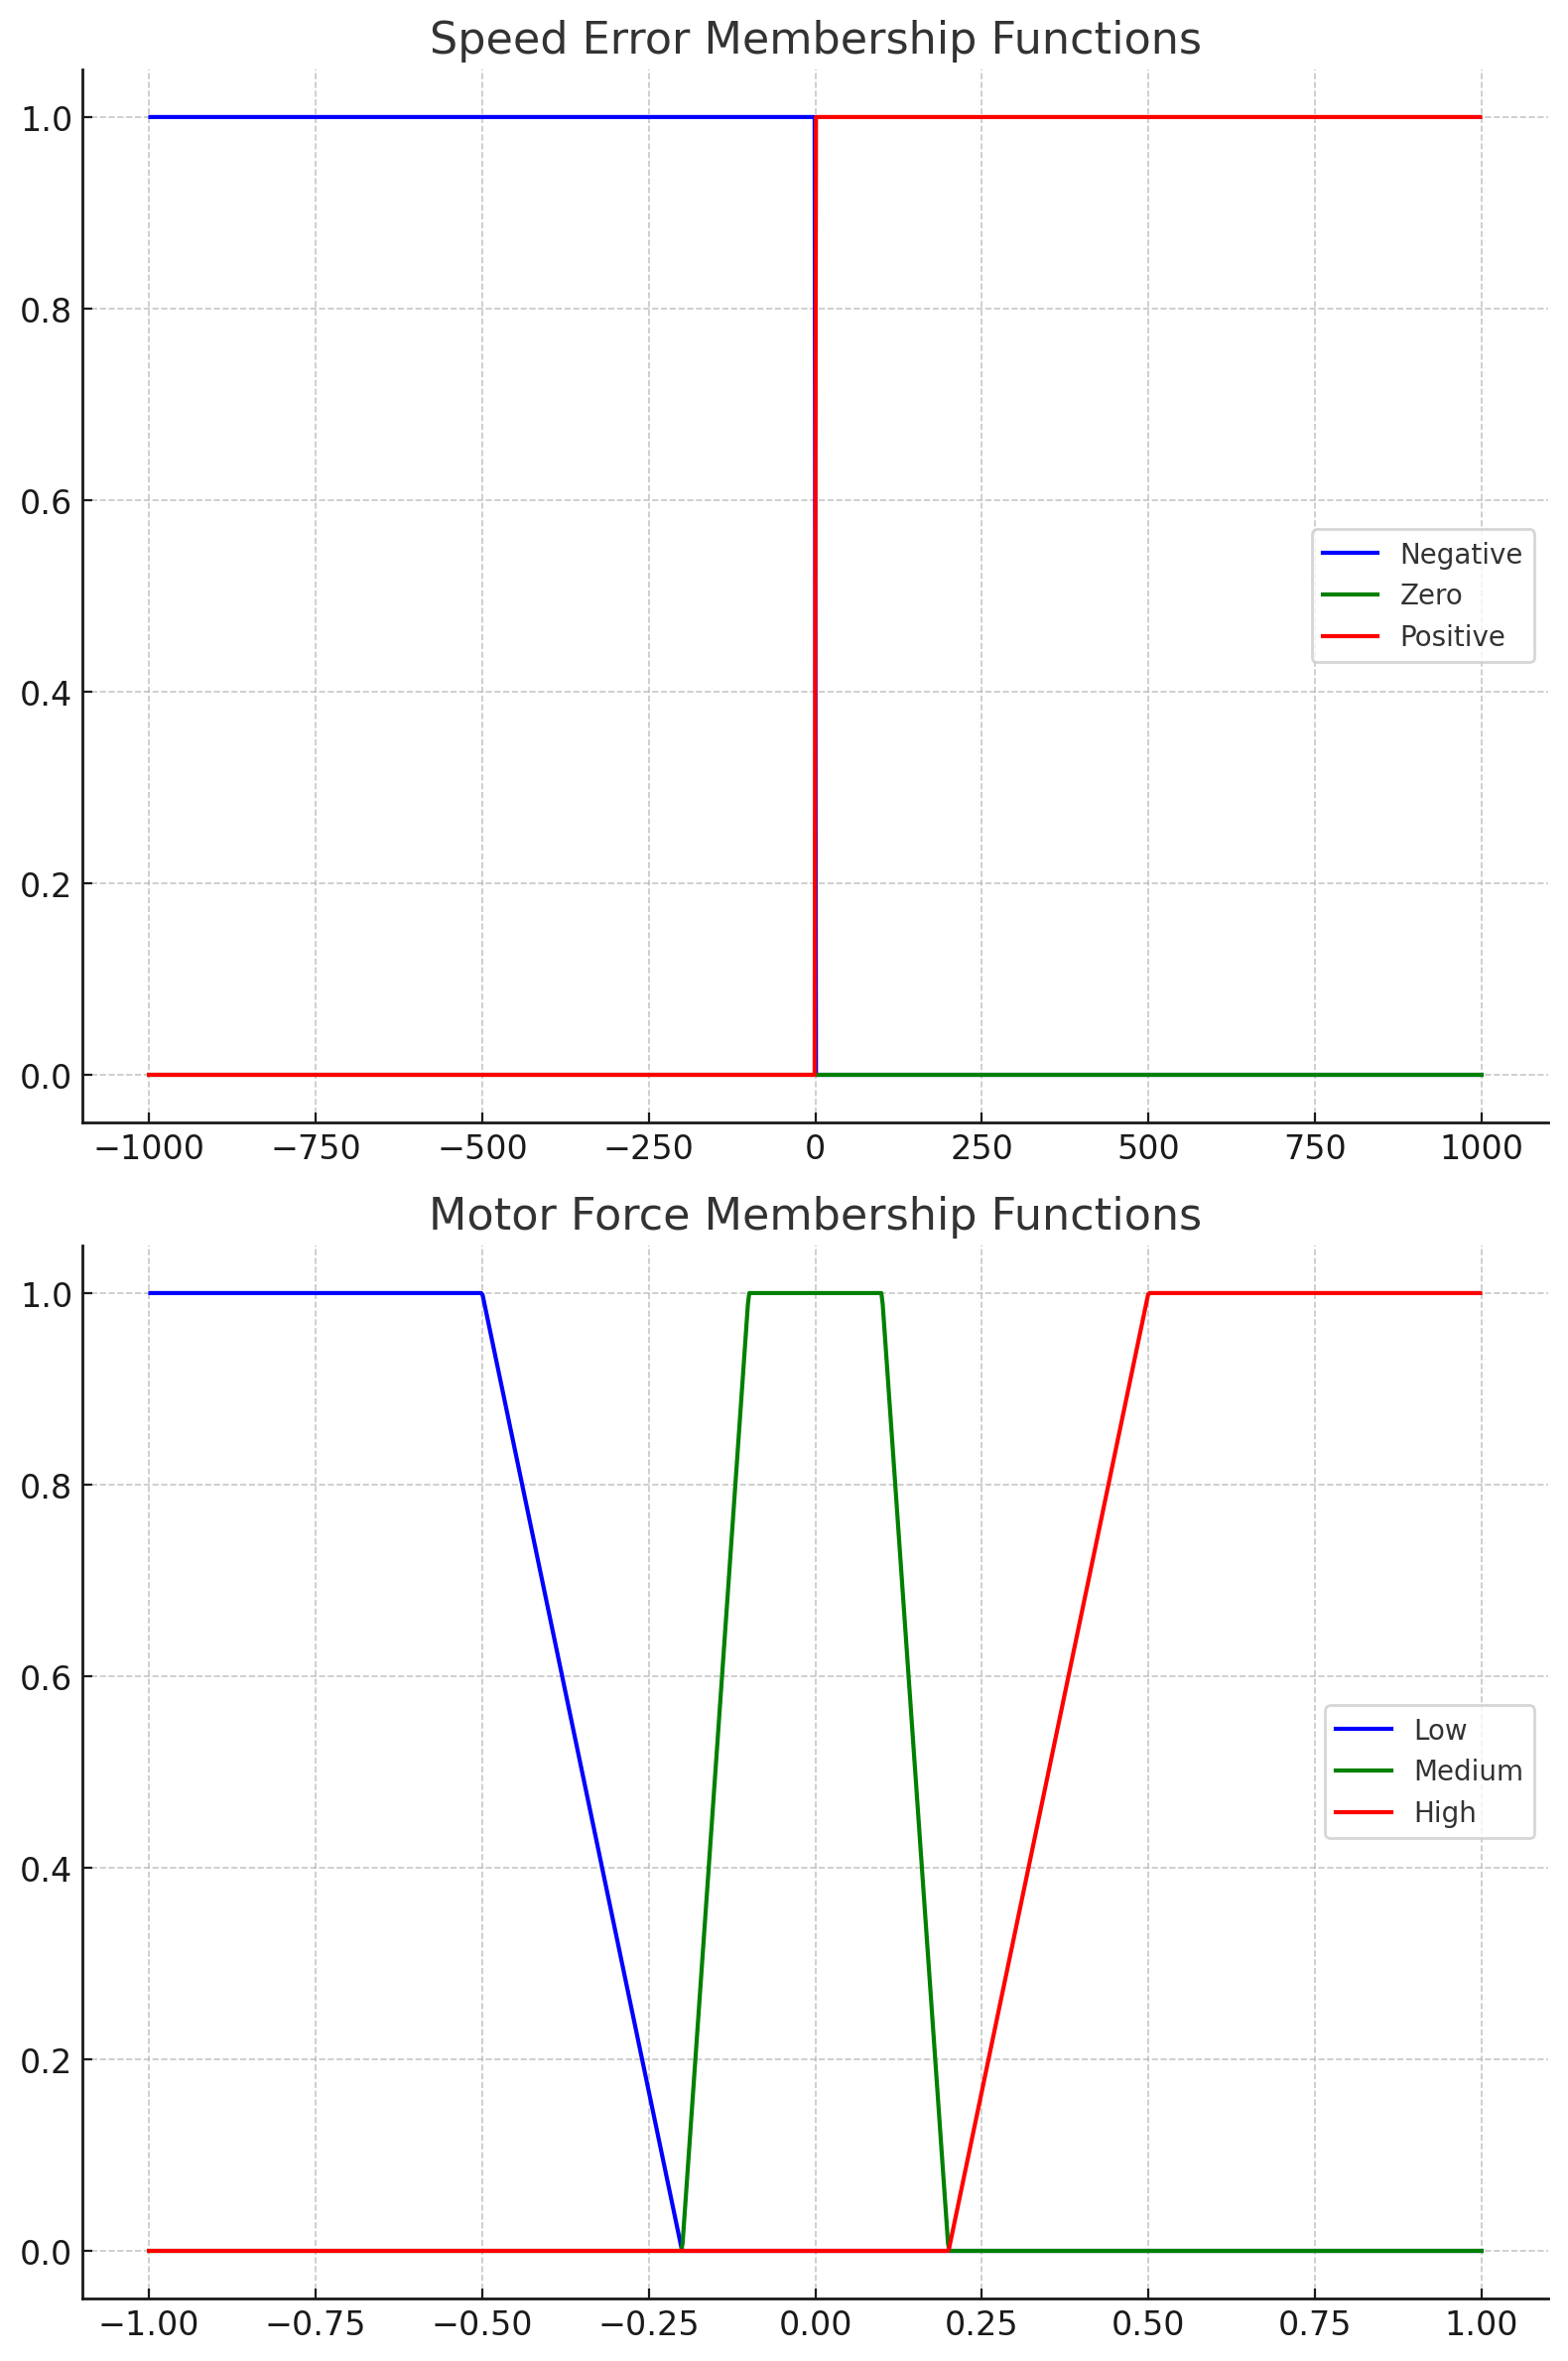
\includegraphics[width=0.9\linewidth]{speed-error-memb.png}
\end{figure}


\clearpage
\section{Θέμα}

\subsection{Ερώτημα}

Το σύστημα είναι:

\begin{equation}
    x(k+1) = h_1(x) \cdot A_1 \cdot x(k) + h_2(x) \cdot A_2 \cdot x(k)
\end{equation}

όπου  
\begin{equation}
    h_1(x) + h_2(x) = 1
\end{equation}
και 

\begin{equation}
    \begin{aligned}
        Α_1 = \begin{bmatrix} 0.9 & a \\ 0 & 0.8 \end{bmatrix}\\
        A_2 = \begin{bmatrix} 0.9 & 0 \\ a & 0.8 \end{bmatrix}
    \end{aligned}
\end{equation}

Για να είναι το σύστημα ευσταθές πρέπει να υπάρχει από κοινού συνάρτηση \eng{Lyapunov}
για καθέναν από τους πίνακες Α. Δηλαδή, πίνακας P συμμετρικός τέτοιος ώστε να ισχύει:

\begin{equation}
    \begin{aligned}
        P > 0 \\
        P \cdot A_1 + A_1 \cdot P < 0 \\
        P \cdot A_2 + A_2 \cdot P < 0 \\
    \end{aligned}
\end{equation}

Παρατηρείται όμως, ότι επειδή:

\begin{equation}
    A_1 = A_2^T
\end{equation}

οι παρακάτω περιορισμοί μπορούν να γραφτούν ως:

\begin{equation}
    \begin{gathered}
        \begin{aligned}
            P > 0 \\
            P \cdot A_1 + A_1 \cdot P < 0 \\
            P \cdot A_2 + A_2 \cdot P < 0 \\
        \end{aligned} \implies
        \begin{aligned}
            P > 0 \\
            P \cdot A_1 + A_2^T \cdot P < 0 \\
            P \cdot A_2 + A_2 \cdot P < 0 \\
        \end{aligned}  \\ \implies
        \begin{aligned}
            P > 0 \\
            P \cdot A_1 + \left(P \cdot A_2 \right)^T < 0 \\
            P \cdot A_2 + A_2 \cdot P < 0 \\
        \end{aligned}
    \end{gathered}
\end{equation}

Δεν συνεχίστηκε η απάντηση του ερωτήματος.

\subsection{Ερώτημα}

Δεν απαντήθηκε.

\end{document}
